\documentclass[12pt]{article}
\usepackage[english]{babel}
\usepackage[utf8]{inputenc}
\usepackage{amsmath, amssymb, amsthm}
\usepackage{graphicx}
\usepackage{hyperref}
\usepackage[margin=.75in]{geometry}
\usepackage{xcolor}
\usepackage{tikz}

\newcommand{\id}{\text{id}}
\newcommand{\od}{\text{od}}

\setlength{\topmargin}{0pt}
\setlength{\headsep}{0pt}
\textheight = 600pt

\title{Branching Heuristics and Pruning Rules for Edge Clique Cover}
\author{Ben Kallus}
\date{Date}

\begin{document}
\maketitle

\section*{Introduction}

\subsection*{Cliques}
    An $n$-clique in an undirected graph $G$ is a subgraph of order $n$ in $G$ in which each vertex is adjacent to each other vertex.
    For example, in the graph $H$ shown in Figure 1, the subgraph induced by the vertices $\{a, b, c\}$ constitutes a 3-clique.
    \begin{center}
        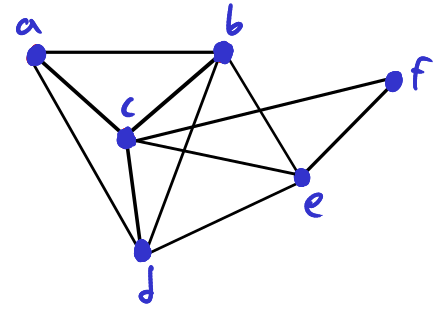
\includegraphics[scale=.6]{fig1.png}

        Figure 1. The graph $H$
    \end{center}

    Note that a clique may be contained in another clique.
    In this case, the 3-clique $\{a, b, c\}$ is a subgraph of the 4-clique $\{a, b, c, d\}$.
    The 4-clique $\{a, b, c, d\}$ is not a subgraph of any other clique in $H$, so we say $\{a, b, c, d\}$ is a maximal clique.

\newpage\subsection*{The Edge Clique Cover Problem}

    An edge clique cover for an undirected graph $G$ is a set of cliques in $G$ with the property that every edge in $G$ is contained in at least one clique in the cover.\footnote{Note that isolated vertices have no effect on an edge clique cover, because they are incident to no edges. Thus, we consider only graphs without isolated vertices.}
    For example, $C_1 = \{\{a, b, c, d\}, \{c, e, f\}, \{d, e\}, \{b, e\}\}$ constitutes an edge clique cover for the graph $H$.
    \begin{center}
        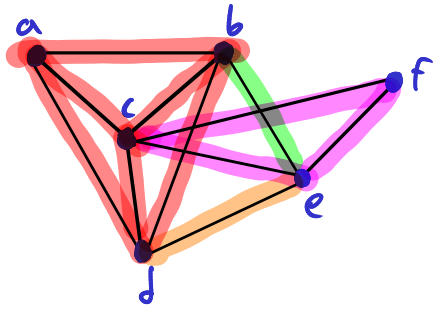
\includegraphics[scale=.6]{fig2.png}

        Figure 2. $H$ shown with its edges colored according to $C_1$
    \end{center}

    Observe that the cover shown in Figure 2 can be made to be smaller; the 2-cliques $\{d,e\}$ and $\{b,e\}$ are both subgraphs of the 3-clique $\{b, d, e\}$, and so a smaller edge clique cover $C_2$ can be constructed by substituting the 2-cliques with the 3-clique.
    \begin{center}
        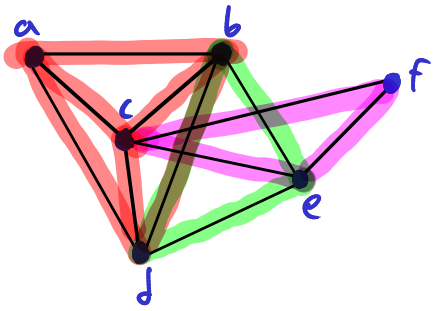
\includegraphics[scale=.6]{fig3.png}

        Figure 3. $H$ shown with its edges colored according to $C_2$
    \end{center}

    In fact, $H$ cannot be covered by any less than 3 cliques, so $C_2$ is a minimum edge clique cover for $H$.
    The edge clique cover number of a graph $G$, $\text{ecc}(G)$, is the number of cliques in a minimum edge clique cover for $G$.
    Note that a graph may have many minimum edge clique covers; $C_3 = \{\{a, b, c, d\}, \{c, e, f\}, \{b, c, d, e\}\}$ is another minimum edge clique cover for $H$.

\newpage\subsection*{Prior Work}

    Although efficient algorithms are known for a few special graph classes, the problem of finding a minimum edge clique cover for a graph in general is NP-complete.
    Approximation algorithms, such as those produced by Conte et al [2018] are known to work well on some real-world networks, but their accuracy is inversely correlated with graph density.
    
    Gramm et al. [2008] developed data reductions for the problem that, employed within a branch-and-reduce algorithm, constitute the state of the art for exactly solving the problem in the general case.
    This branch-and-reduce algorithm works by applying simple data reduction rules.
    For example, for a graph $G$ with a degree-1 vertex $u$, $\text{ecc}(G) = \text{ecc}(G - u) + 1$.
    Thus, when computing $\text{ecc}(G)$, degree-1 vertices can be repeatedly scanned for and removed until none remain, leaving a reduced graph $G'$ such that $\text{ecc}(G) = \text{ecc}(G') + (|G| - |G'|)$.
    Gramm et al. introduce two other polynomial-time reduction rules that either reduce the size of the input graph or identify a clique that must be present in a minimum edge clique cover for the input graph.
    Once all of these reductions no longer apply, a search tree algorithm is employed.
    First, an an uncovered edge $e$ is selected from the reduced graph, and the set $C = \{C_1, C_2, \hdots, C_k\}$ consisting of all maximal cliques containing $e$ is computed.
    Then for each clique $c \in C$, the algorithm recursively solves for the smallest edge clique cover containing $c$, applying reductions as it goes, until every edge in the graph is covered.
    Since each edge in the reduced graph must be contained in some clique in an edge clique cover, it is clear that the smallest among these covers is a minimum edge clique cover.

    An error is present in the third reduction rule described by Gramm et al.
    The rule reads ``Consider a vertex $v$ that has at least one prisoner. If each prisoner is connected to at least one vertex other than $v$ via an uncovered edge (note that this is automatically given when the instance is reduced with respect to Rules 1 and 2), and the prisoners dominate the exits, then delete $v$. To reconstruct a solution for the unreduced instance, add $v$ to every clique containing a prisoner of $v$."
    As written, this reduction is invalid.
    A counterexample is shown below.

    \begin{center}
        Here will be a graphic that shows a counterexample for Rule 3 as written.
        Because the smallest counterexample I have found for Rule 3 so far is a graph with 9 vertices, the graphic is too large to fit on one page, so I'm trying to think of a better counterexample.
    \end{center}

    To make Rule 3 correct, an extra condition must hold: the prisoners must dominate the exits via uncovered edges.

\newpage\section*{Pruning}
    
    We introduce pruning rules to the branch-and-reduce algorithm from Gramm et al.

    \textbf{Lemma 1.} Let $M$ be an independent set of vertices in an undirected graph $G$. Then, $\text{ecc}(G) \geq |M|$.
    \begin{proof}
        Let $M$ be an independent set of vertices in an undirected graph $G$.
        Then, no two vertices in $M$ are adjacent, and so no two vertices in $M$ can belong to the same clique in an edge clique cover for $G$.
        Thus, any edge clique cover for $G$ must contain at least one clique for every vertex in $M$, so $$\text{ecc}(G) \geq |M|.$$
    \end{proof}

    Once the branch-and-reduce algorithm has found an edge clique cover of (not necessarily minimum) size $k$ for a graph $G$, \textbf{Lemma 1} can be used to prune the search tree.
    Suppose that an independent set of size $i$ is found in the reduced graph $G'$.
    If any branch of the search tree for $G'$ leads to a partial cover consisting of at least $k-i$ cliques, then no further computation in that branch is necessary because the resulting cover will not be smaller than the current best found so far.

    \textbf{Lemma 2.} Let $S$ be an independent set of edges in an undirected graph $G$ such that the subgraph of $G$ induced by the endvertices of these edges is $K_4$-free. Then, $\text{ecc}(G) \geq |S|$.
    \begin{proof}
        Let $S$ be an independent set of edges in an undirected graph $G$ such that the subgraph of $G$ induced by the endvertices of the edges in $S$ is $K_4$-free.
        Because $S$ is an independent set of edges in $G$, the edges in $S$ do not share any endvertices.
        Thus, there is no triangle in $G$ containing two edges in $S$.
        Consider $G'$, the subgraph of $G$ induced by the endvertices of the edges in $S$.
        Because $G'$ is $K_4$-free, it must be that for each pair of distinct edges $e_1 = v_1v_2, e_2 = v_3v_4 \in S$, $G$ does not contain at least one of $v_1v_3, v_1v_4, v_2v_3, v_2v_4$.
        Then, no two edges in $S$ can belong to the same clique in an edge clique cover for $G$, so $$\text{ecc}(G) \geq |S|.$$
    \end{proof}

    \textbf{Lemma 2} enables search tree pruning in exactly the same way as \textbf{Lemma 1}.
    Further pruning can be applied using the maximum of the bounds described in the two lemmas.
    
    The approximation algorithm described by Conte et al. never underestimates $\text{ecc}(G)$ on an input graph $G$.
    Thus, Conte's algorithm provides an initial upper bound suitable for beginning pruning immediately, which removes the need to wait until a leaf in the search tree has been found.
    Additionally, by repeatedly applying Conte's algorithm, if the cover computed by Conte's algorithm is ever smaller than the best cover with the search tree, then that bound can be used instead.

\newpage\section*{Implementation}

    Branching heuristics:
        - lowest score edge
        - random edge
        - highest score edge
        - choose with probability

    pruning:
        - size of max independent set
        - size of max edge set such that their vertices induce a K4-free subgraph of G.
            Strategies for constructing this set:
                - Pick edges in random order
                - Presort adjlists by degree
                - Presort adjlists by degree of neighborhood
                - Presort, then sort again
        - Using Conte for initial upper bound
        - Using Conte throughout

\section*{Experiments}

    Which branching heuristics work best?
        Try lowest score, highest score, random edge, and some kind of choice with probability

    Which pruning techniques produce the best bound?
        Try IS, and edge set
        Try running Conte throughout

    What are the best methods for constructing the edge set used for pruning?
        - Presorting methods (degree, degree of neighbors)
        - Sorting in the middle
    
\end{document}
